% Copyright 2004 by Till Tantau <tantau@users.sourceforge.net>.
%
% In principle, this file can be redistributed and/or modified under
% the terms of the GNU Public License, version 2.
%
% However, this file is supposed to be a template to be modified
% for your own needs. For this reason, if you use this file as a
% template and not specifically distribute it as part of a another
% package/program, I grant the extra permission to freely copy and
% modify this file as you see fit and even to delete this copyright
% notice. 

% \UseRawInputEncoding
\documentclass{beamer}

% There are many different themes available for Beamer. A comprehensive
% list with examples is given here:
% http://deic.uab.es/~iblanes/beamer_gallery/index_by_theme.html
% You can uncomment the themes below if you would like to use a different
% one:
%\usetheme{AnnArbor}
%\usetheme{Antibes}
%\usetheme{Bergen}
%\usetheme{Berkeley}
%\usetheme{Berlin}
%\usetheme{Boadilla}
%\usetheme{boxes}
%\usetheme{CambridgeUS}
%\usetheme{Copenhagen}
%\usetheme{Darmstadt}
%\usetheme{default}
%\usetheme{Frankfurt}
%\usetheme{Goettingen}
%\usetheme{Hannover}
%\usetheme{Ilmenau}
%\usetheme{JuanLesPins}
%\usetheme{Luebeck}
\usetheme{Madrid}
%\usetheme{Malmoe}
%\usetheme{Marburg}
%\usetheme{Montpellier}
%\usetheme{PaloAlto}
%\usetheme{Pittsburgh}
%\usetheme{Rochester}
%\usetheme{Singapore}
%\usetheme{Szeged}
%\usetheme{Warsaw}

\usepackage{pgfgantt}
\usepackage{todonotes}
\usepackage{media9}
\usepackage{subfigure}
\usepackage{booktabs,array}
\usepackage[font=tiny,labelfont=bf]{caption}
\usepackage{tabulary}
\usepackage{caption}
\usepackage{graphicx}
\usepackage{siunitx}
\usepackage{arydshln}
\usepackage{rotating}


% Customize Warsaw color 
\setbeamercolor*{palette primary}{use=structure,fg=white,bg=red!50!black}
\setbeamercolor*{palette secondary}{use=structure,fg=white,bg=red!60!black}
\setbeamercolor*{palette tertiary}{use=structure,fg=white,bg=red!70!black}

% Customize Warsaw block title and background colors
\setbeamercolor{block title}{bg=red!50!black,fg=white}

\setbeamertemplate{navigation symbols}{} % Remove navigation symbols
\setbeamertemplate{bibliography item}{\insertbiblabel}  % insert bibliography numbers instead of symbol
\setbeamertemplate{caption}[numbered] % adds the figure or table number to the caption.

% Set up footer manually
\setbeamertemplate{footline}
{
  \leavevmode%
  \hbox{%
  \begin{beamercolorbox}[wd=.45\paperwidth,ht=2.25ex,dp=1ex,center]{author in head/foot}%
    \usebeamerfont{author in head/foot}\insertshortauthor\hspace*{1em}(\insertshortinstitute)
  \end{beamercolorbox}%
  \begin{beamercolorbox}[wd=.4\paperwidth,ht=2.25ex,dp=1ex,center]{title in head/foot}%
    \usebeamerfont{title in head/foot}\insertshorttitle
  \end{beamercolorbox}%
  \begin{beamercolorbox}[wd=.15\paperwidth,ht=2.25ex,dp=1ex,center]{date in head/foot}%
    \usebeamerfont{date in head/foot}\insertframenumber{} / \inserttotalframenumber
  \end{beamercolorbox}}%
  \vskip0pt%
}

%==============================================================================
%     TITLE
%==============================================================================
\title[Smart Robotic Cart]{Smart Robotic Cart: A Prototype}

\author[K.~Allen, D.~Beebe, J.~Braker]{Kallistah~Allen \and Darrah~Beebe \and Jason~Braker
Advisors:~Dr.~Suruz~Miah \and Dr.~Prasad~Shastry}
% - Give the names in the same order as the appear in the paper.
% - Use the \inst{?} command only if the authors have different
%   affiliation.

\institute[Bradley University] % (optional, but mostly needed)
{
  Department of Electrical and Computer Engineering\\
  Bradley University\\
  1501 W. Bradley Avenue\\
  Peoria, IL, 61625, USA
}
% - Use the \inst command only if there are several affiliations.
% - Keep it simple, no one is interested in your street address.

\date[April~20,~2021]{Tuesday, April~27,~2021}

% - Either use conference name or its abbreviation.
% - Not really informative to the audience, more for people (including
%   yourself) who are reading the slides online

\logo{\hfill\href{http://www.bradley.edu}{
\includegraphics[width=0.75cm]{figs/logoBU1-Print}}}  % place logo in every page 


\subject{Mobile Robot Localization}
% This is only inserted into the PDF information catalog. Can be left
% out. 

% If you have a file called "university-logo-filename.xxx", where xxx
% is a graphic format that can be processed by latex or pdflatex,
% resp., then you can add a logo as follows:

% \pgfdeclareimage[height=0.5cm]{university-logo}{university-logo-filename}
% \logo{\pgfuseimage{university-logo}}

% Delete this, if you do not want the table of contents to pop up at
% the beginning of each subsection:
\AtBeginSection[]
{
  \begin{frame}<beamer>{Outline}
    \tableofcontents[currentsection,currentsubsection]
  \end{frame}
}

%==============================================================================
%==============================================================================
%     START OF SLIDES
%==============================================================================
%==============================================================================

% Let's get started
\begin{document}

\begin{frame}
  \titlepage
\end{frame}

\begin{frame}{Outline} 
  \tableofcontents%[pausesections]
  % You might wish to add the option [pausesections]
\end{frame}

% Section and subsections will appear in the presentation overview
% and table of contents.
\section{Introduction}

\begin{frame}{Introduction}{}
 % \begin{center}
 %    \href{videos/smartRoboticCartIntroVideo.mp4}{\includegraphics[width=0.8\textwidth]{figs/img/finalPresVideoTitle.png}}
 %  \end{center}
\end{frame}

\begin{frame}{Introduction}{Problem Statement}
  \begin{block}{Problem Statement}
    \begin{LARGE}
      Design a robotic cart that follows the user without line of sight (LoS) sensors
    \end{LARGE}
  \end{block}
  \pause
  \begin{block}{Proposed Solution}
    \begin{LARGE}
      Utilize wireless radio frequency (RF) signal strength to locate and then follow the user
    \end{LARGE}
  \end{block}
\end{frame}

%----------------------------------


%----------------------------------

\begin{frame}{Introduction}{Previous Work}
  \begin{block}{Existing Solution}
        Mobile application platform interface with ultrasound and radio transmission technology~\cite{Sales2016-CompaRob}
  \end{block}
    % \begin{figure}[b]
    %     \centering
    %     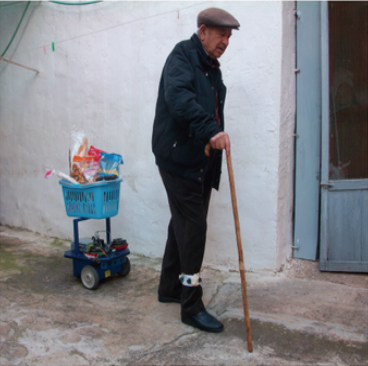
\includegraphics[width=0.4\textwidth]{figs/img/CompaRob}
    %     \caption{CompaRob}
    %     %\label{fig:sysBlockDiag}
    % \end{figure}
\end{frame}

%----------------------------------

\begin{frame}{Introduction}{Previous Work}
  \begin{block}{Existing Solution}
        Gated Recurrent Unit (GRU) network with LiDAR sensor and camera to map the customer~\cite{islam_lam_fukuda_kobayashi_kuno_2019}
  \end{block}
    % \begin{figure}[b]
    %     \centering
    %     \includegraphics[width=0.38\textwidth]{figs/img/ShoppingSuportRobot}
    %     \caption{Shopping Support Robot}
    %     %\label{fig:sysBlockDiag}
    % \end{figure}
\end{frame}

%----------------------------------


%------------------------------------------------------------------------------
%     SECTION BREAK
%------------------------------------------------------------------------------

\section{Conclusions and Future Work}

\begin{frame}{Conclusions and Future Work}
  \begin{block}{Conclusions}
    \begin{itemize}
      \item The algorithm we implemented works the majority of the time
      \item Through tests and gathering data we were able iterate on our approach and tune the algorithms to function more reliably
      \item Our design is cost effective in comparison to other robotic carts
    \end{itemize}
  \end{block}
  \begin{block}{Future Work}
    \begin{itemize}
      \item Improve the localization algorithm for better angle estimation
      \item Test more reflector designs to see if the XBee signals can be more refined
      \item Implement obstacle detection and avoidance
      \item Multi-frequency radio modules to try to improve distance estimation
    \end{itemize}
  \end{block}
\end{frame}

%------------------------------------------------------------------------------
%     SECTION BREAK
%------------------------------------------------------------------------------

\section{References}

\begin{frame}{References}
  \bibliographystyle{IEEEtran}
  \bibliography{bib/references.bib}
\end{frame}

%==============================================================================
%==============================================================================
%     END OF SLIDES
%==============================================================================
%==============================================================================

\end{document}

%%% Local Variables:
%%% mode: latex
%%% TeX-master: t
%%% End:
